% AY2013 制御工学 解答例
% 回答の流れ・言葉遣いは 03_制御工学/参考/「制御工学Ⅱ（完成版）」に寄せる。
% デザイン（囲み枠等）は真似しない。解答・数値は本年度過去問から自力で導いた。
\documentclass[11pt,a4paper]{article}
\usepackage{../../../00_common/preamble}

\usetikzlibrary{positioning,arrows.meta,calc}
\usepackage{pgfplots}
\pgfplotsset{compat=newest}

\title{制御工学 AY2013 解答例（専門応用科目I）}
\author{}
\date{}

\begin{document}
\maketitle

% ==================================================================
\section*{第1問（50点）}

一自由度振動系（質量 $m$、粘性係数 $d$、バネ定数 $k$、力 $f(t)$、変位 $x(t)$）について答える。
運動方程式は
\[
  m\ddot{x}+d\dot{x}+kx=f(t).
\]

\subsection*{(1) 伝達関数}
初期値ゼロでラプラス変換して
\begin{align*}
  &\qquad (ms^2+ds+k)\,X(s)=F(s)\\
  &\therefore\quad \frac{X(s)}{F(s)}=\frac{1}{ms^2+ds+k}.
\end{align*}
\[
  \therefore\quad \ans{\;G(s)=\dfrac{1}{ms^2+ds+k}\;}
\]

\subsection*{(2) 定常値が $2$ になる $k$}
$m=1$, $d=1$ とし、単位ステップ入力 $F(s)=\dfrac1s$ を加える。安定なので最終値の定理より
\begin{align*}
  &\qquad x(\infty)=\lim_{s\to0}sX(s)=\lim_{s\to0}\frac{1}{s^2+s+k}=\frac{1}{k}\\
  &\therefore\quad \frac{1}{k}=2.
\end{align*}
定常値は $d$ によらず $1/k$ で決まる。
\[
  \therefore\quad \ans{\;k=\dfrac12\;}
\]

\subsection*{(3) 無減衰系の単位ステップ応答}
$m=1$, $d=0$, $k=1$、初期値ゼロ、$F(s)=\dfrac1s$ なので
\begin{align*}
  &\qquad G(s)=\frac{1}{s^2+1}\\
  &\therefore\quad X(s)=\frac{1}{s(s^2+1)}=\frac1s-\frac{s}{s^2+1}\\
  &\therefore\quad x(t)=\mathcal{L}^{-1}[X(s)]=1-\cos t.
\end{align*}
$d=0$ ゆえ減衰せず、$x(t)$ は $1$ を中心に振幅 $1$ で持続振動する（$0\le x\le 2$、周期 $2\pi$）。
\[
  \therefore\quad \ans{\;x(t)=1-\cos t\;}
\]

\begin{center}
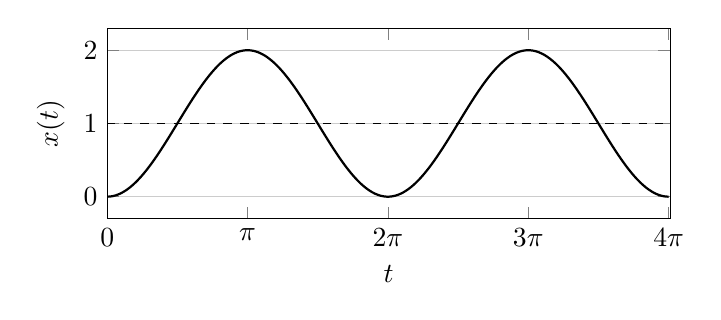
\begin{tikzpicture}
\begin{axis}[
  width=0.72\linewidth, height=4cm,
  xmin=0, xmax=12.6, ymin=-0.3, ymax=2.3,
  xlabel={$t$}, ylabel={$x(t)$},
  xtick={0,3.1416,6.2832,9.4248,12.566},
  xticklabels={$0$,$\pi$,$2\pi$,$3\pi$,$4\pi$},
  ytick={0,1,2}, ymajorgrids=true, grid style={gray!40},
]
\addplot[thick,domain=0:12.566,samples=200]{1-cos(deg(x))};
\addplot[dashed,domain=0:12.566]{1};
\end{axis}
\end{tikzpicture}
\end{center}

\subsection*{(4) 自由応答}
$m=1$, $d=1$, $k=1$、$x(0)=1$, $\dot{x}(0)=0$、$f(t)=0$。自由振動の方程式は
\begin{align*}
  &\qquad \ddot{x}+\dot{x}+x=0
   \quad\therefore\quad s^2+s+1=0
   \quad\therefore\quad s=-\frac12\pm\frac{\sqrt3}{2}j.
\end{align*}
減衰振動 $x(t)=\e^{-t/2}\!\left(A\cos\frac{\sqrt3}{2}t+B\sin\frac{\sqrt3}{2}t\right)$ とおき、初期条件を入れる。
\begin{align*}
  &\qquad x(0)=A=1\\
  &\qquad \dot{x}(0)=-\frac12A+\frac{\sqrt3}{2}B=0
   \quad\therefore\quad B=\frac{1}{\sqrt3}.
\end{align*}
\[
  \therefore\quad \ans{\;x(t)=\e^{-t/2}\!\left(\cos\tfrac{\sqrt3}{2}t+\tfrac{1}{\sqrt3}\sin\tfrac{\sqrt3}{2}t\right)\;}
\]
極の実部が負なので $t\to\infty$ で $x\to0$。よって定常値は存在し $\ans{\;x(\infty)=0\;}$。

\bigskip
\noindent 検算: (3) は極 $\pm j$（無減衰の持続振動）、(4) は導いた $x(t)$ が $\ddot x+\dot x+x=0$ と
初期条件 $x(0)=1,\ \dot x(0)=0$ を満たすことを SymPy で確認✓。

\newpage
% ==================================================================
\section*{第2問（50点）}

$K_0$ と $G_1(s)$ を直列接続した系を考える。全体の伝達関数は
\[
  G(s)=K_0\,G_1(s)=\frac{2}{10s^2+12.5s+2}.
\]

\subsection*{(1) ゲインと位相}
$s=j\omega$ を代入する。分母は $(2-10\omega^2)+12.5\,j\omega$ だから
\begin{align*}
  &\qquad |G(j\omega)|=\frac{2}{\sqrt{(2-10\omega^2)^2+(12.5\omega)^2}},\\
  &\qquad \angle G(j\omega)=-\tan^{-1}\!\frac{12.5\,\omega}{\,2-10\omega^2\,}.
\end{align*}
\[
  \therefore\quad \ans{\;|G(j\omega)|=\dfrac{2}{\sqrt{(2-10\omega^2)^2+(12.5\omega)^2}},\quad
  \angle G(j\omega)=-\tan^{-1}\dfrac{12.5\omega}{2-10\omega^2}\;}
\]

\subsection*{(2) ゲイン線図（漸近線）}
分母を因数分解すると、極は実数 $s=-0.188,\ -1.062$（$\zeta>1$ の過減衰）。
時定数形に直すと
\[
  G(s)=\frac{1}{(1+5.31s)(1+0.94s)},\qquad |G(0)|=1=0\,\mathrm{dB}.
\]
よって折れ点は $\omega\simeq0.19$ と $\omega\simeq1.06\,[\mathrm{rad/s}]$、傾きは
$\omega<0.19$ で $0$、$0.19<\omega<1.06$ で $-20$、$\omega>1.06$ で $-40\,[\mathrm{dB/dec}]$。

\begin{center}
\begin{tikzpicture}
\begin{axis}[
  width=0.86\linewidth, height=5.2cm,
  xmin=1e-2, xmax=1e2, ymin=-100, ymax=20, xmode=log,
  xlabel={$\omega\,[\mathrm{rad/s}]$}, ylabel={ゲイン [dB]},
  ytick={-100,-80,-60,-40,-20,0,20},
  xmajorgrids=true, ymajorgrids=true, xminorgrids=true,
  grid style={line width=0.3pt, draw=gray!60},
  extra y ticks={0}, extra y tick style={grid=major, grid style={line width=1pt, draw=black}},
  legend pos=south west, clip=true, enlargelimits=false,
]
% 漸近線: 0dB→(0.188)→-20→(1.062)→-40
\addplot[thick] coordinates {(0.01,0) (0.188,0) (1.062,-30) (100,-148.6)};
\addlegendentry{漸近線}
% 真値
\addplot[thick,dashed] coordinates
  {(0.01,0.0) (0.1,-0.7) (0.188,-3.0) (0.5,-13.2) (1.062,-26.0) (10,-66.0) (100,-145.0)};
\addlegendentry{真値}
\node[anchor=south] at (axis cs:0.188,0) {\scriptsize $\omega=0.19$};
\node[anchor=north east] at (axis cs:1.062,-30) {\scriptsize $\omega=1.06$};
\end{axis}
\end{tikzpicture}
\end{center}

\subsection*{(3) 単位ステップ応答}
$G(s)$ の極が実数（過減衰）なので、$X(s)=\dfrac{G(s)}{s}$ を部分分数分解して
\begin{align*}
  &\qquad X(s)=\frac{2}{s(10s^2+12.5s+2)}
   =\frac{1}{s}-\frac{1.216}{s+0.188}+\frac{0.216}{s+1.062}\\
  &\therefore\quad x(t)=\mathcal{L}^{-1}[X(s)]
   =1-1.216\,\e^{-0.188t}+0.216\,\e^{-1.062t}.
\end{align*}
過減衰なのでオーバーシュートなく単調に立ち上がり、定常値 $1$ に収束する。
\[
  \therefore\quad \ans{\;x(t)=1-1.216\,\e^{-0.188t}+0.216\,\e^{-1.062t}\;}
\]

\begin{center}
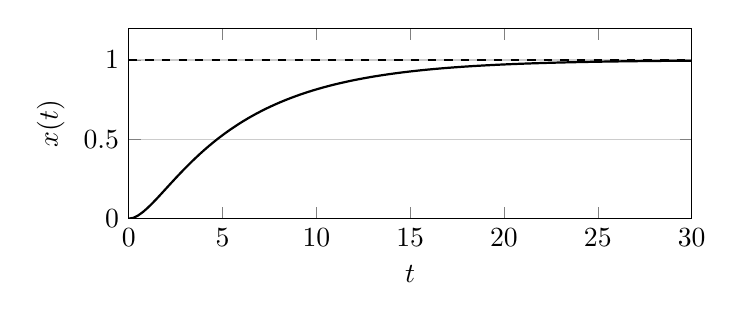
\begin{tikzpicture}
\begin{axis}[
  width=0.72\linewidth, height=4cm,
  xmin=0, xmax=30, ymin=0, ymax=1.2,
  xlabel={$t$}, ylabel={$x(t)$},
  ytick={0,0.5,1}, ymajorgrids=true, grid style={gray!40},
]
\addplot[thick,domain=0:30,samples=120]{1-1.216*exp(-0.188*x)+0.216*exp(-1.062*x)};
\addplot[dashed,domain=0:30]{1};
\end{axis}
\end{tikzpicture}
\end{center}

\subsection*{(4) 過渡特性・定常特性の考察}
\begin{itemize}\setlength{\itemsep}{1pt}
  \item \textbf{過渡特性}：極が実数 2 個（$\zeta>1$ の過減衰）なので、(3) のとおり振動・
        オーバーシュートを生じない。応答の速さは絶対値の小さい極 $s=-0.188$（時定数
        $\simeq5.3\,$s）が支配し、整定は遅い。
  \item \textbf{定常特性}：(2) より直流ゲイン $0\,\mathrm{dB}$（$|G(0)|=1$）。本系は積分器を
        含まない 0 型なので、単位ステップ入力に対し定常値は $1$ となり、誤差そのものは
        ゲインで決まる（速度入力などには定常偏差が残る）。
\end{itemize}
\[
  \therefore\quad \ans{\;\text{過減衰で無振動・整定が遅く、0 型ゆえステップ定常値は }1\;}
\]

\bigskip
\noindent 検算: $G(0)=1$、極 $s=-0.188,-1.062$（実数・過減衰 $\zeta\approx1.40$）、
ステップ応答は $x(0)=0,\ x(\infty)=1$ で単調増加であることを数値確認✓。

\end{document}
